\lecture{11}{lun 01 mag 2023 17:17}{Guadagno e costante di tempo, sistemi del primo ordine}
	\lablsection{Guadagno e costante di tempo}
	\twomini{\[G(s) = \frac{\mu}{s^g}\frac{\prodc_i(1+s\tau_i)}{\prodc_k(1+sT_k)}\]}{\[
		\begin{aligned}
			\text{Zeri}&:-\frac{1}{\tau_i}\\
			\text{Poli}&: -\frac{1}{T_k}
		\end{aligned}
		\]}
	Per quanto riguarda il guadagno $ \mu $ valuto due sotto casi
	\begin{enumerate}
		\item \emph{Guadagno statico}\\$ g=0 \to \mu = \lim_{s\to0}G(s) \approx G(o)$
		\\Capiamo di cosa si tratta:
		\twomini{\[\begin{cases}
				\dot{x} = Ax+Bu\\
				y = Cx+Du
			\end{cases}\]}{\[G(s)=C(sI-A)^-1B+D\]}
		Valuto il sistema all'equilibrio dato $ u = \overline{u}\,\, t\geq0 $
		\begin{equation*}
			\begin{cases}
				\overline{x} = -A^{-1} B\overline{u}\\
				\overline{y} = -CA^{-1}\overline{u} + D\overline{u} =\left( -CA^{-1} + D\overline{u}\right)
			\end{cases}
		\end{equation*}
		Scrivo $ G(0) = -CA^{-1}B + D $, quindi $ \mu = \frac{\overline{y}}{\overline{u}} $ e cioè il guadagno statico è il rapporto tra uscita ed ingresso all'equilibrio.
		\item \emph{Guadagno semplice o generalizzato} $ g\neq 0 \to \mu = \lim_{s\to0} s^gG(s)$
	\end{enumerate}
	\lablsubsection{Risposte Canoniche}
	I parametri (o indici) caratteristici della risposta allo scalino: vedremo funzioni del primo o del secondo ordine.
	\nota{Valuteremo il moto forzato. La stabilità del sistema non dipende dagli ingressi}
	Disegniamo un generico segnale:
	\begin{figure}[H]
		\centering
		\includegraphics[width=0.7\linewidth]{Images/generico_segnale}
	\end{figure}
	Nel quale:
	\begin{itemize}
		\item $ T_s $: tempo di salita: è il tempo che il segnale impiega per passare da $ 0.1y_{\infty} $ a $ 0.9y_{\infty} $, con $ y_{\infty} $ il valore del segnale a transitorio esaurito.
		\item $ T_{a_{\epsilon}} $: tempo di assestamento al $ (100\pm\epsilon)\% $ di $ y_\infty $, è il tempo impiegato dal segnale per entrare nella striscia $ \pm\epsilon\% $ di $ y_\infty $.
		\item $ S $: massima sovra elongazione.
		\item $ S_\% =\frac{ \displaystyle\max_\tau \left[ y (\tau)\right] - y_\infty }{ y_\infty }$ massima sovra elongazione percentuale. 
	\end{itemize}
	\lablsection{Sistemi del primo ordine}
	\begin{enumerate}
		\item $ G(s) $ strettamente propria (cioè grado del denominatore è 1 mentre del numeratore è 0)
		\begin{enumerate}
			\item[\textbf{a.}] $ g=0 \to G(s) = \frac{\mu}{sT+1}$, polo: $ \frac{-1}{T} $
			$ G(s) $ è A.S. quando $ T>0 $.
			\begin{itemize}
				\item Risposta allo scalino ($ u(t) = \operatorname{sca}(t) \to U(s) = \frac{1}{s} $)
				\begin{equation*}
					Y(s) = G(s) \frac{1}{s} = \frac{\mu}{s(sT+1)}
				\end{equation*}
				Antitrasformo e trovo
				\begin{equation*}
					y(t) = \mu (1-\exp^{-t/T}) \quad t\geq0 \qquad \dot{y}(0) =\frac{\mu}{T}
				\end{equation*}
				\twomini{
					\begin{figure}[H]
						\centering
						\includegraphics[width=0.7\linewidth]{Images/risp_scalino1}
				\end{figure}}{Più T è piccolo, più veloce sarà la risposta}
				Sto assumendo per semplicità $ \mu>0 $ ma è anche possibile che $\mu$ sia negativo. In questo caso il grafico si specchia sull'asse delle ascisse.\\\\
				Usando il \emph{TVF} (\cref*{subsec:Teorema del valore finale (TVF)}) con (T>0) trovo:
				\begin{equation*}
					\displaystyle\lim_{t\to\infty} y(t) = \lim_{s\to0} sY(s) = \mu
				\end{equation*}
				A transitorio esaurito ho un valore pari a $\mu$. Il tempo di assestamento è pari a 
				\begin{equation*}
					T_{a\epsilon} =4.6T 
				\end{equation*}
				\item\emph{risposta all'impulso}
				\begin{equation*}
					u(t) =\operatorname{imp}(t) \to U(s)
					Y(s) = G(s) \cdot 1=\frac{\mu}{sT +1}
				\end{equation*}
				Antitrasformo e trovo
				\begin{equation*}
					y(t) = \frac{\mu}{T}\exp^{-t/T} \quad t\geq 0
				\end{equation*}
				\nota{La risposta all'impulso è la derivata della risposta allo scalino}
				\begin{center}
					\begin{tikzpicture}
						\begin{axis}[
							axis lines = left,
							xlabel = $t$,
							ylabel = $y$,
							no markers,
							xticklabel = \empty,
							yticklabel = \empty]
							\addplot+ [smooth,decorate,red]{e^-x};
							\addlegendentry{$T>0\, G(s)$ A.S.}
						\end{axis}
					\end{tikzpicture}
				\end{center}
				\item \emph{$g = 1$ $G(s) = \frac{\mu}{s}$}
				\item \emph{Risposta allo scalino}\\
				$Y(s) = G(s) \cdot \frac{1}{s} = \frac{\mu}{s^2}$
				Antitrasformo $y(t) = \mu \cdot\operatorname{ram}(t)$\\
				\begin{center}
					\begin{tikzpicture}
						\begin{axis}[
							axis lines = left,
							xlabel = $t$,
							ylabel = $y$,
							no markers,
							xticklabel = \empty,
							yticklabel = \empty]
							\addplot{x};
						\end{axis}
					\end{tikzpicture}
				\end{center}
				\item \emph{Risposta all'impulso}\\
				$Y(s) = G(s) \cdot 1 = \frac{\mu}{s}$\\
				La risposta è uno scalino di ampiezza $\mu$.\\
				$y(t) = \mu\operatorname{sca}(t)$\\
				\begin{center}
					\begin{tikzpicture}
						\begin{axis}[axis lines = left,
							xlabel = $t$,
							ylabel = $y$,
							no markers,
							xticklabel = \empty,
							yticklabel = \empty]
						\end{axis}
					\end{tikzpicture}
				\end{center}
			\end{itemize}
			\item $G(s)$ proprie $\operatorname{grad}(D(s))=\operatorname{grad}(N(s))=1$
			  \subitem $g=0$ $G(s) = \mu \\frac{1+st}{1+sT}$
			  Antitrasformo
			  \[y(t) = \mu (1 +(\frac{t}{T}-1)\exp^{\\frac{-t}{T}}) \quad t\geq0\]
			  Assumo $\mu>0 , T>0 $ (\gls{as})\\
			  Ora non resta che da capire cosa succede al variare di $t$.
			  % TODO: add graphs
			  Osservazioni:\\
			  \begin{itemize}
				\item La risposta all'impulso è la derivata della risposta allo scalino: $y(t) = \frac{\mu}{T}(\frac{t}{T}-1)\exp^{\frac{-t}{T}}$
				\item Nei primi due casi con $t>0$, la risposta \textit{anticipa}, quella del caso senza zero.
				\item Quando $t<0$ il sistema si dice a fase non minima
			  \end{itemize}
			  \item $g=1$ $G(s) = \mu \frac{st+1}{s}$
				\subitem Risposta allo scalino
				\[Y(s) = G(s) \cdot \frac{1}{s} = \frac{\mu}{s^2}(st+1)\]
				Antitrasformo
				\[y(s) = \mu t +\mu \operatorname{ram}(t)\quad t\geq0\]
				Assumo $\mu>0$
				%% TODO: add graphs
				\item $g=-1$ $G(s) = \mu \frac{s}{1+st}$
				  \subitem Risposta allo scalino
				  \[Y(s) = G(s)\frac{\mu}{st+1}\]
				  Noto che è uguale alla risposta all'impulso di una $G(s)$ strettamente propria con $g=0$
				 % TODO: copy graph from file
		\end{enumerate}
	\end{enumerate}
	\lablsubsection{Sistemi del secondo ordine}
	\begin{enumerate}
	  \item Poli reali e nessuno zero
		\twomini{\[G(s) = \frac{\mu}{(1+sT_1)(1+sT_2)}\]}{Poli: $- \frac{1}{T_1} $ , $- \frac{1}{T_2}$ \\\gls{as} $T_1,T_2 >0$}
		\subitem Risposta allo scalino
		\[Y(s) = G(s) \cdot \frac{1}{s} = \frac{\mu}{s(1+sT_1)(1+T_2) \quad \mu>0}\]
		Applico i teoremi \gls{tvi} e \gls{tvf}
		\[y(0) = \liminf_{s \to \infty} sY(s) = 0\]
		\[\dot{y}(0) = \liminf_{s \to \infty} s\underbrace{(sY(s) - y(0))}_{\L[\dot{y(t)}]} = 0 \]
		\[\ddot{y}(0) = \liminf_{s \to \infty} s\underbrace{(s^2Y(s) - \dot y(0))}_{\L[\ddot{y}(t)]} = \frac{\mu}{T_1 T_2}>0 \]
		\[y(\infty) = \limsup_{s \to 0} sY(s) = \mu\]
		Applico Heaviside
		\[y(t) = \mu \left[1 - \frac{T_1}{T_1 - T_2} \exp^{\frac{-t}{T_1}}+\frac{T_2}{T_1 - T_2} \exp^{\frac{-t}{T_1}}\right] \quad t\geq 0\]
		% Todo: inserisci grafico
		Noto che $T_1 \simeq T_2 $ vuol dire che i poli si influenzano reciprocamente, se una delle due $T$ è più grande, allora
		domina sull'altra e posso approssimare la $G(s)$ come una funzione del primo ordine.
		\begin{equation*}
		 T_1 >> T_2 \to y(t) \simeq \mu (1- \exp^{\frac{-t}{T_1}})
		\end{equation*}
		Analogalmente per $T_2 >> T_1$. Il tempo di assestamento sarà circa $4,6 T_i \quad T_i>>T_j$.\\
		Nota: se $T_1 =T_2 =T$, il tempo di assestamento è $T_{a1} = 6,664T$
		\item Poli reali e uno zero
		  \[G(s) = \mu \frac{(1+st)}{(1+sT_1)(1+sT_2)}\quad \begin{aligned}
			\mu >0\\
			T_1,T_2 >0
		  \end{aligned} \]
		  \subitem Risposta allo scalino
		  \[Y(s) = G(s) \frac{1}{s} = \frac{\mu}{s}\frac{(1+st)}{(1+sT_1)(1+sT_2)}\]
		  Applico \gls{tvi} e \gls{tvf} e trovo
		  \[y(0) = 0 \quad,\quad \dot y(0) = \frac{\mu t}{T_1T_2}\quad,\quad y(\infty) = \mu\]
		  %TODO: inserisci grafici
		  \item Poli complessi coniugati
		\begin{equation*}
			G(s) = \mu \frac{\omega_n^2}{s^2 +2\xi\omega_ns +\omega_n^2}
			\qquad\qquad 
			\begin{aligned}
				&\mu >0\\
				&\omega_n: \text{Pulsazione naturale}\\
				&\xi: \text{Smorzamento}
			\end{aligned}
		\end{equation*}
			\subitem Risposta allo scalino
			\[y(0) = 0 \quad,\quad \dot y(0) = \frac{\mu t}{T_1T_2}\quad,\quad \ddot y(0)=\mu\omega_n^1>0\\y(\infty) = \mu\]
			Antitrasformo
			\[y(t)=\mu\left[1- \frac{1}{\sqrt{1-\xi^2}}\exp^{-\xi\omega_nt}\sin(\omega_n\sqrt{1-\xi^2}t+\alpha)\right]\quad t\geq0\]
			Con $\xi = \cos(\alpha)$\\
			Noto che $\xi=0$ significa che ci sono due poli coniugati a parte reale nulla.
			\[y(t) = \mu [1-\cos(\omega_nt)]\]
			\begin{tikzpicture}
			  \begin{axis}[
			  	axis lines = middle,
			  	xlabel = $t$,
			  	ylabel = $y$,
			  	no markers,
			  	xticklabel = \empty,
			  	yticklabel = \empty,
			  	xmin=0,
			  	xmax= 4*pi,
			  	ymax=1.1]
				\addplot[red,domain=0:4*pi,samples=200]{cos(deg(x))};
			  \end{axis}
			\end{tikzpicture}\\
			Considero ora $\xi > 0 $: La risposta è compresa tra due funzioni esponenziali:\\
			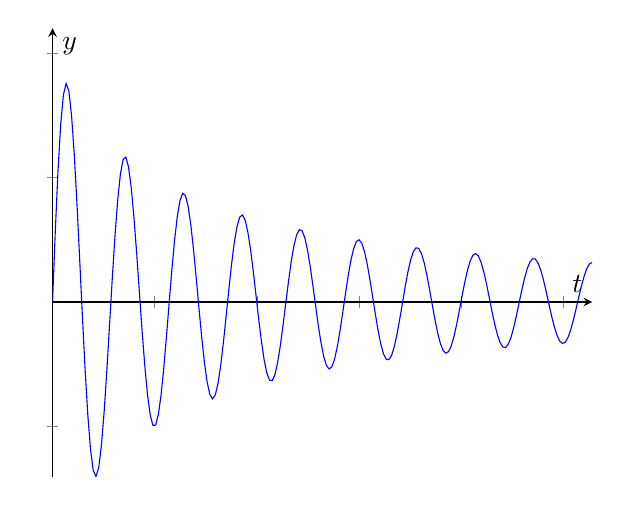
\begin{tikzpicture}
			  \begin{axis}[
			  	axis lines = middle,
			  	xlabel = $t$,
			  	ylabel = $y$,
			  	no markers,
			  	xticklabel = \empty,
			  	yticklabel = \empty,
			  	xmin=1,
			  	xmax= 2*pi,
			  	ymax=1.1]
				\addplot[blue,domain=1:2*pi,samples=200]{1/x * cos(deg(x)*11)};
				%todo: errore in questo grafico
			  \end{axis}
			\end{tikzpicture}\\
			Sovra-elongazione massima percentuale: $S_\%=100\cdot \exp^{(\frac{-\xi\pi}{\sqrt{1-\xi^2}})} $
			Le sovra-elongazione dipendono da $\xi$: più alto è $\xi$ maggiore è lo smorzamento
			%todo: aggiugi grafico
			Troviamo il tempo di assestamento $(\varepsilon=1)$ prendo un inviluppo esponenziale
			\[\mu (1-\exp^{-\xi\omega_nT_{a1}})=0.99\mu \to \xi \omega_nT_{a1} = h 100\]
			\[T_{a1} = \frac{\ln(100)}{\xi\omega_n}\simeq \frac{4.6}{\xi\omega_n}\]
	\end{enumerate}
%%% Local Variables:
%%% mode: latex
%%% TeX-master: "master"
%%% End:
